\subsection{Incident Journal Sequencing (M2)}
\label{sec:protocol-m2}

M2 provides sequencing, and it does not depend on responder reachability. Only the
command edge assigns positions to decisions, so the journal has one total order. It
accepts each \textit{client\_event\_id} once and assigns \textit{event\_seq} atomically
with the journal insert; a duplicate folds onto its existing entry rather than taking a
new number. Consumers replay the journal in \textit{event\_seq} order, so materialized
state is rebuildable from it. A decision enters the incident record when the command
edge sequences it; it survives a later promotion only if it reaches the core first
(\S~\ref{sec:protocol-m4}).

\subsection{Durable Outbox and Idempotent Submission (M3)}
\label{sec:protocol-m3}

For R1 and R2, M3 gives responders a safe local path before the command edge is
reachable: field submissions are locally durable, idempotent, and eventually forwarded
to the incident journal (Figure~\ref{fig:outbox-sequence}). The boundary is between
local durability and the command edge's commit. A responder may acknowledge local
acceptance after the outbox insert, but marks an item forwarded only after the command
edge accepts it or recognizes a duplicate.

\begin{figure}[!t]
\centering
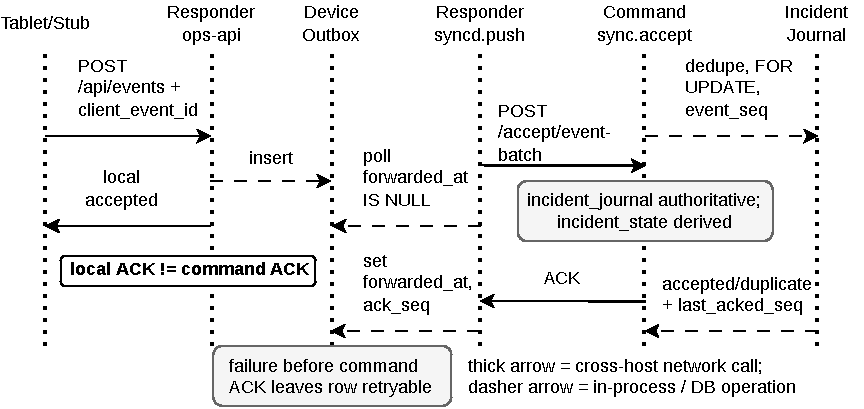
\includegraphics[width=\columnwidth]{figures/fig_outbox_sequence.drawio.pdf}
\caption{Responder outbox protocol is the steady-state field-submission path from tablet to incident journal. The journal assigns the authoritative sequence number, and duplicate delivery is handled by \textit{client\_event\_id}.}
\label{fig:outbox-sequence}
\end{figure}

The M3 contract has three parts:
\begin{enumerate}
  \item Each submission has a globally unique idempotency key, \textit{client\_event\_id}, scoped by the incident and originating client identity.
  \item A responder accepts a submission only after the event is stored in its local outbox.
  \item A responder may mark an outbox item forwarded only after the command edge acknowledges durable incident-journal acceptance or duplicate recognition.
\end{enumerate}

Outbox delivery is at least once and is deduplicated at the command edge; there is no
claim of causal ordering across independent responder outboxes before the command edge
orders them.

\subsection{Fenced Promotion (M4)}
\label{sec:protocol-m4}

M4 moves the command role and provides authority. There is no autonomous failover: an
operator decides that command moves, and M4 keeps the core's journal single-writer
across the move.

\textit{Epochs and the holder check.} The regional core issues each command tenure an
epoch, per incident; the edge taking authority does not choose it. Core issuance gives
promotions on independent vehicles a single order, since each edge owns its database and
an edge-local counter cannot distinguish two edges that both believe they lead. The
epoch is a fencing token in the usual sense~\cite{kleppmann2017ddia}. Every journal
entry carries its epoch, and the core accepts forwarded entries only from the node
recorded as holding the current epoch. Checking the node, not only the number, matters
because a demoted edge that reconnects can read the current epoch from the core. The
check is a protocol boundary, not authentication (\S~\ref{sec:non-claims}).

\textit{Promotion.} The operator first confirms that the old command edge is
unreachable. The candidate then copies the journal prefix held by the core and verifies
that it is contiguous; the core issues the next epoch, and its insert orders concurrent
attempts; only then does the role change. Promotion therefore needs the candidate to
reach the core, but it does not wait for the old command edge.

\textit{The lease.} A cut-off former command edge cannot learn that its epoch is stale,
so it must stop by itself. Write authority is a lease~\cite{gray1989leases} renewed at
the core, on traffic and on an idle heartbeat. A command edge that has not reached the
core for the lease length $L$ stops accepting decisions: on a timer, not on being told.

\begin{figure}[t]
\centering
% Promotion while the command edge is cut off: the case M4 has to handle.
% Hand-drawn TikZ rather than a plot -- the message is the order of events and
% where each entry ends up, which is a layout property, not a data property.
% Colours follow main.tex: accepting path blue (accept), refusal orange (fence).
\begin{tikzpicture}[
  x=1cm, y=1cm,
  font=\scriptsize,
  lane/.style={draw=black!60, line width=0.6pt},
  idle/.style={draw=black!25, line width=0.6pt},
  cutlane/.style={draw=black!45, line width=0.6pt, dash pattern=on 2pt off 1.5pt},
  fenced/.style={draw=fence, line width=1.6pt},
  entry/.style={circle, fill=accept, inner sep=1.2pt},
  msg/.style={-{Latex[length=1.5mm,width=1.2mm]}, draw=accept, line width=0.6pt},
  nak/.style={-{Latex[length=1.5mm,width=1.2mm]}, draw=fence, line width=0.6pt},
  tmark/.style={draw=black!30, densely dotted},
]
% Overlap window: after B is promoted and before A's lease lapses.
\fill[fence!12] (3.1,-0.18) rectangle (5.3,1.95);
\node[color=fence!85!black] at (4.2,2.17) {A and B both accept};

% Time marks.
\foreach \x/\t in {1.3/{$t_0$}, 3.1/{$t_1$}, 5.3/{$t_0{+}L$}, 6.9/{$t_2$}} {
  \draw[tmark] (\x,-0.3) -- (\x,1.95);
  \node[anchor=north] at (\x,-0.3) {\t};
}

% Lane labels.
\node[anchor=east, font=\scriptsize\bfseries] at (0.5,1.7) {A};
\node[anchor=east, font=\scriptsize\bfseries] at (0.5,0.85) {core};
\node[anchor=east, font=\scriptsize\bfseries] at (0.5,0.0) {B};

% Lane A: connected, cut off but accepting, lease lapsed, demoted.
\draw[lane]    (0.6,1.7) -- (1.3,1.7);
\draw[cutlane] (1.3,1.7) -- (5.3,1.7);
\draw[fenced]  (5.3,1.7) -- (8.5,1.7);
\node[color=black!55] at (1.95,1.5) {cut off};
\node[entry] (x) at (2.5,1.7) {};
\node[above=0.5pt] at (x.north) {X};
\node[entry] (z) at (4.6,1.7) {};
\node[below=0.5pt] at (z.south) {Z};
\node[color=fence!85!black] at (6.1,1.93) {lease lapsed};
\node[color=fence!85!black] at (7.75,1.93) {demoted};

% Core lane.
\draw[lane] (0.6,0.85) -- (8.5,0.85);
\node[anchor=north] at (8.05,0.78) {$1..k$, Y};

% Lane B: responder until promoted at t1, then command edge.
\draw[idle] (0.6,0.0) -- (3.1,0.0);
\draw[lane] (3.1,0.0) -- (8.5,0.0);
\node[entry] (y) at (3.8,0.0) {};
\node[above=0.5pt] at (y.north) {Y};

% Promotion at t1: B copies the core's prefix and receives epoch e+1.
\draw[msg] (3.17,0.78) -- (3.17,0.08);
\node[anchor=east] at (3.07,0.43) {prefix $1..k$, epoch $e{+}1$};
% B forwards Y.
\draw[msg] (3.95,0.07) -- (4.35,0.78);

% Reconnection at t2: A forwards X, the core refuses, A demotes itself.
\draw[msg] (6.97,1.62) -- (7.17,0.93);
\node[anchor=east] at (7.02,1.22) {X, Z};
\draw[nak] (7.45,0.93) -- (7.65,1.62);
\node[anchor=west, color=fence!85!black] at (7.62,1.22) {409};
\end{tikzpicture}

\caption{Promotion while the command edge A is cut off, with lease length $L$. A is cut
off at $t_0$ and keeps accepting decisions, such as X, that it cannot forward. At $t_1$
an operator promotes B: B copies the core's prefix $1..k$, receives epoch $e{+}1$, and
accepts Y. Until A's lease lapses at $t_0{+}L$, both edges accept (shaded), and A
accepts Z. When A reconnects at $t_2$, the core refuses X and Z with HTTP~409 and A
demotes itself. The core's journal holds $1..k$ and Y; X and Z stay on A.}
\label{fig:promotion-timeline}
\end{figure}

\textit{What M4 guarantees.} In Figure~\ref{fig:promotion-timeline}, B takes authority
at once while A accepts until its lease lapses, so for up to $L$ both edges accept
decisions. The core's journal still never takes entries from two holders, and the
refused edge demotes itself and raises an operator alert. What A accepted but never
forwarded stays on A: decisions from its legitimate tenure (X) as well as from the
overlap (Z). Neither is merged, so the incident record is incomplete until an operator
reviews them.

\textit{Choosing $L$.} The same lease stops a legitimate command edge that has lost only
its backhaul, so $L$ sets \systemname{}'s position in the trade-off of
\S~\ref{sec:tradeoff}. A longer lease keeps decisions flowing through longer outages; a
shorter one narrows the window in which two edges accept. The prototype uses $L=90$\,s
by default. Waiting out the old lease before promotion would close the window, at the
cost of delaying each such promotion by up to $L$ (\S~\ref{sec:alternatives}).
